% 1977 年广西百色卷（理科）第三题：圆 O 内两弦 AB、CD 相交于 E，
% 虚线 AC、BD 为证 △AEC∽△DEB 所连（按源卷第 3 页布局）
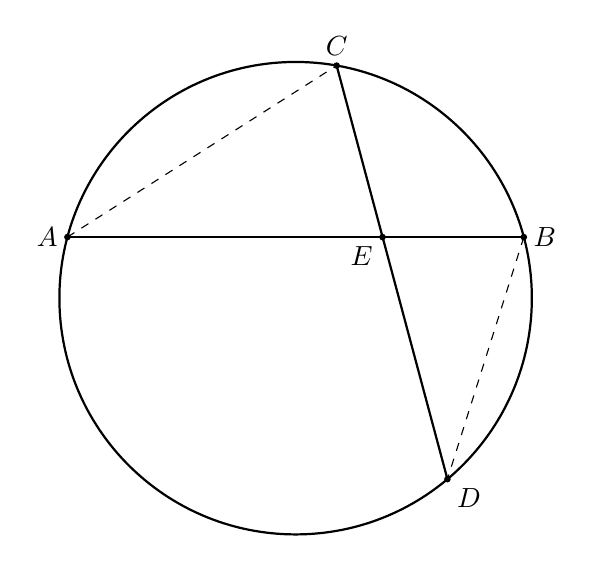
\begin{tikzpicture}[scale=1.0]
  % 圆半径 3cm；A 在 165°、B 在 15°、C 在 80°、D 在 310°
  \draw[thick] (0,0) circle (3);
  \coordinate (A) at (-2.898,0.776);
  \coordinate (B) at (2.898,0.776);
  \coordinate (C) at (0.521,2.954);
  \coordinate (D) at (1.928,-2.298);
  \coordinate (E) at (1.104,0.776); % AB 与 CD 的交点
  \draw[thick] (A)--(B);
  \draw[thick] (C)--(D);
  \draw[dashed] (A)--(C);
  \draw[dashed] (B)--(D);
  \fill (A) circle (1.2pt) node[left] {$A$};
  \fill (B) circle (1.2pt) node[right] {$B$};
  \fill (C) circle (1.2pt) node[above] {$C$};
  \fill (D) circle (1.2pt) node[below right] {$D$};
  \fill (E) circle (1.2pt) node[below left] {$E$};
\end{tikzpicture}
